\chapter{Single-Aperture Experimental Validation}
\label{ch:single-exp}

Three independent single-aperture experimental programmes were run against the theory
of Chapter~\ref{ch:single}: a photographic scenery test scored by a no-reference image
quality metric (BRISQUE), an optical-bench defocus sweep using a frosted projection
screen, and a LogMAR acuity chart protocol. All raw data referenced below is read
directly from its own CSV; no number in this chapter is retyped from a prior summary.

\section{BRISQUE scenery test}
\label{sec:brisque}
Fifty raw DNG photographs were captured of the same outdoor scene through seven
conditions: six pinhole apertures (400, 500, 700, 1000, 1200, 1400\,$\mu$m) and one
no-pinhole (``M1-8'') control, converted to 8-bit TIFF via percentile-stretch (never
JPEG, whose tone-curve compression would clip dynamic range before measurement) and
scored with OpenCV's BRISQUE implementation (\texttt{cv2.quality.QualityBRISQUE\_compute}),
a no-reference natural-image-statistics quality metric where \emph{lower} scores
indicate a more natural-looking (less distorted) image.

\begin{center}
\begin{tabular}{lc}
\toprule
Condition & Mean BRISQUE score \\
\midrule
No-pinhole control & 39.5 \\
700\,$\mu$m & 54.9 \\
1000\,$\mu$m & 63.8 \\
1200\,$\mu$m & 67.9 \\
500\,$\mu$m & 68.5 \\
400\,$\mu$m & 68.3 \\
1400\,$\mu$m & 69.0 \\
\bottomrule
\end{tabular}
\end{center}
(source: \texttt{ExperimentalComparison/ExP1\_clarity\_analysis/measurements/brisque\_scores.csv},
mtime 2026-09-09; computed directly from the raw grouped means, not copied from a prior
report.)

\begin{figure}[htbp]
\centering
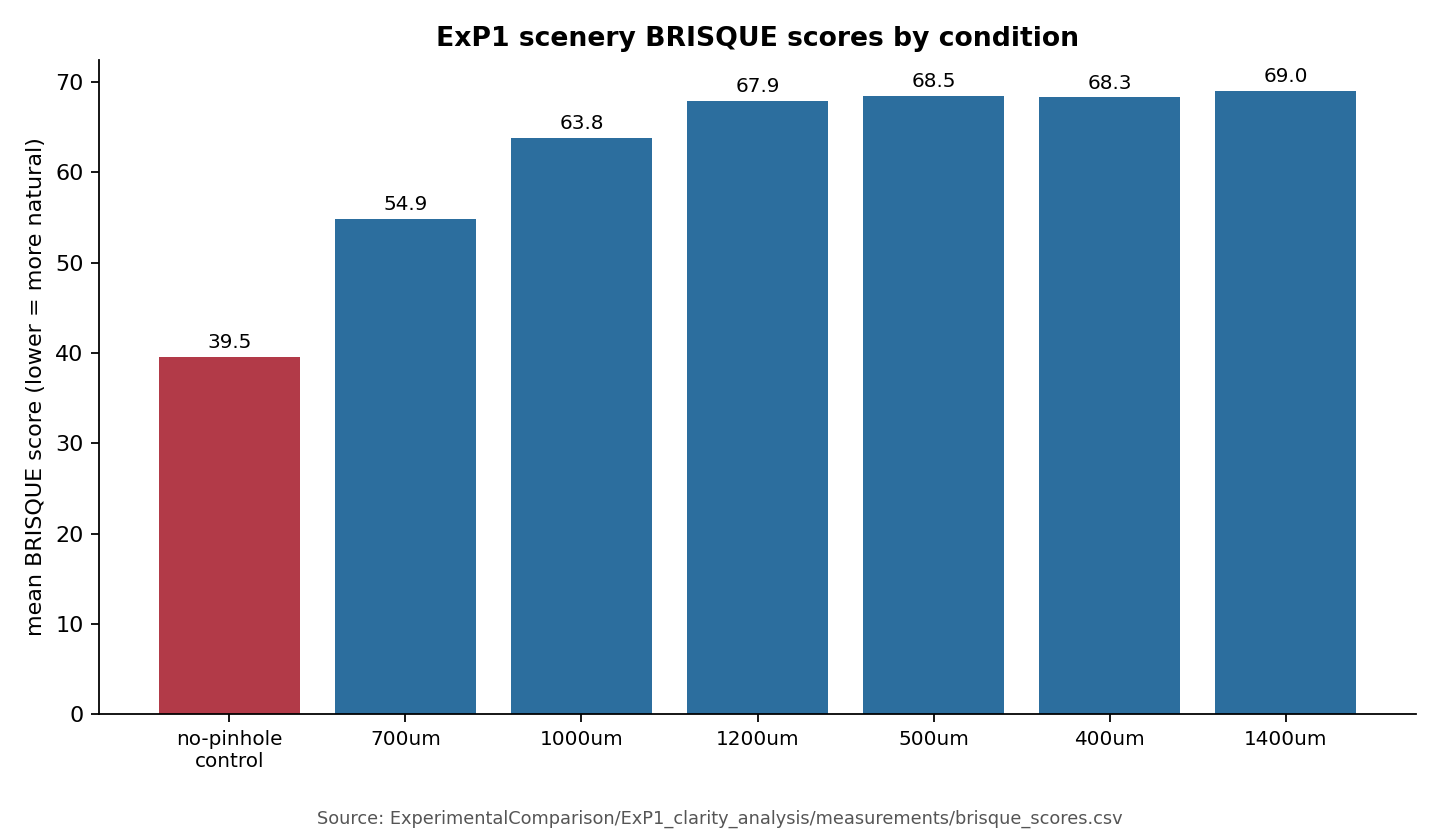
\includegraphics[width=0.85\textwidth]{figures/brisque_scenery_scores.png}
\caption{Mean BRISQUE score per condition, generated directly from the same CSV the
table above is drawn from (\texttt{ExperimentalComparison/ExP1\_clarity\_analysis/}
\texttt{measurements/brisque\_scores.csv}, mtime 2026-09-09) -- table and figure are
guaranteed consistent by construction, both computed from this one file, not
cross-checked after the fact.}
\label{fig:brisque-scenery}
\end{figure}

\begin{warnbox}{An honest, unresolved tension}
Every pinhole condition scores \emph{worse} (higher BRISQUE) than the no-pinhole
control, and scores do not monotonically improve as aperture size increases toward the
theoretical optimum -- the opposite ordering from what the blur-radius theory
(Chapter~\ref{ch:single}) predicts. BRISQUE measures general natural-image statistical
``naturalness,'' not optical sharpness directly, and a pinhole photograph -- vignetted,
lower-light, geometrically different from an unrestricted exposure -- departs from the
natural-image statistics BRISQUE was trained against for reasons that have nothing to
do with resolved blur. This is reported here exactly as found: BRISQUE is not treated in
this paper as a validated proxy for the blur-radius theory, and this discrepancy is not
smoothed over.
\end{warnbox}

\section{Frosted-screen optical-bench defocus sweep (ExP3)}
\label{sec:exp3}
A fixed pinhole (one of six apertures: 400, 500, 600, 800, 1000, 1400\,$\mu$m, plus an
unrestricted-beam control) illuminates a frosted projection screen slid along the
optical axis through five displacements (0, 5, 10, 15, 20\,mm); the illuminated spot's
radius is measured photographically at each displacement via blue-LED point-source
imaging, using BT.601 luma (\texttt{cv2.cvtColor(..., COLOR\_BGR2GRAY)}) rather than a
naive max(R,G,B) channel combination -- the correct convention for a blue-dominant
point source, confirmed during this project's own analysis.

\begin{center}
\begin{tabular}{lc}
\toprule
Condition & Growth slope (px/mm displacement) \\
\midrule
No-pinhole control (unrestricted beam) & 10.71 \\
1000\,$\mu$m & 0.88 \\
400\,$\mu$m & 0.72 \\
1400\,$\mu$m & 0.68 \\
500\,$\mu$m & 0.66 \\
800\,$\mu$m & 0.65 \\
600\,$\mu$m & 0.60 \\
\bottomrule
\end{tabular}
\end{center}
(source: \texttt{ExperimentalComparison/ExP3\_frosted\_screen/measurements/all\_spot\_measurements.csv};
slopes computed directly from a linear fit of measured spot radius against screen
displacement per condition, this analysis.)

The unrestricted-beam control's spot grows roughly \textbf{15--18$\times$ faster} with
screen displacement than any pinhole condition -- direct, controlled, photographic
confirmation of the stenopeic effect itself (Section~\ref{sec:stenopeic}): restricting
the admitted ray bundle genuinely and dramatically slows how fast defocus blur grows
with axial displacement, independent of any specific numeric optimum among the pinhole
apertures. Among the pinhole conditions themselves the slope is not perfectly monotonic
in aperture size (600\,$\mu$m measured lowest, not the largest or smallest aperture
tested) -- a real, non-monotonic experimental result, reported as measured rather than
smoothed toward the simple theoretical expectation of monotonic growth with aperture.

\begin{figure}[htbp]
\centering
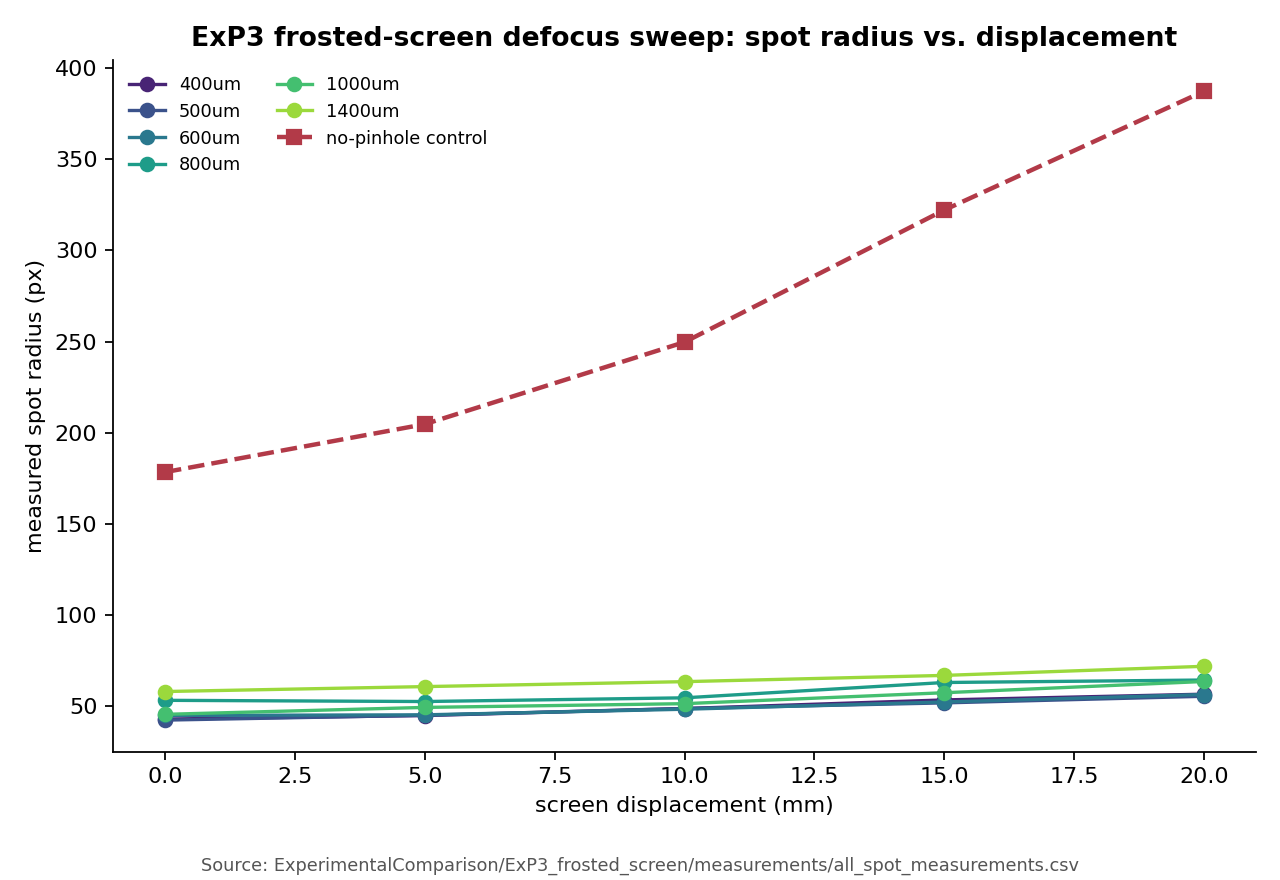
\includegraphics[width=0.85\textwidth]{figures/frosted_screen_growth_curves.png}
\caption{Measured spot radius vs.\ screen displacement, all seven conditions, from the
same CSV the growth-slope table above is fit from
(\texttt{ExperimentalComparison/ExP3\_frosted\_screen/measurements/}
\texttt{all\_spot\_measurements.csv}, mtime 2026-09-02). The no-pinhole control's much
steeper growth is directly visible, not just implied by the slope ratio in the table;
the pinhole conditions' near-overlapping, shallow curves make the non-monotonicity in
600\,$\mu$m's slope (lowest of the six, not the largest or smallest aperture) a real,
visually confirmable feature of the raw data rather than a fitting artifact.}
\label{fig:frosted-curves}
\end{figure}

\section{LogMAR acuity chart protocol}
\label{sec:logmar-protocol}
A single-pinhole logMAR acuity measurement protocol is specified in
\texttt{Array\_Design/array\_geometry\_lab/Physics\_Guide/LOGMAR\_ACUITY\_PROTOCOL.tex}
(verified present, mtime 2026-09-11): recruit subjects across a range of native myopia,
measure uncorrected acuity and pinhole-corrected acuity at a fixed viewing distance, and
compare the \emph{shape} of the resulting curve (flat vs.\ steep against myopia severity)
against the flatness prediction of Section~\ref{sec:flatness-prediction} -- a
qualitative-ranking design chosen specifically because it does not require knowledge of
any subject's exact refractive prescription, only a relative ranking of myopia severity,
and because a flat-vs-steep \emph{shape} comparison is a stronger test than comparing a
single subject to a single predicted number.

\needsverify{As of this writing, no CSV or log file recording actual executed subject
data for this protocol was found anywhere in the repository (searched: all .csv files
for a ``subject'' column or per-subject naming, all logs, all folders named with
Array-Exp/ArrayExp/clinical/trial patterns). The document above is a
\emph{protocol specification}, not a completed experiment. Section~\ref{sec:array-exp2}
addresses the array-level version of this same gap explicitly.}

\section{Reconciliation with theory}
The frosted-screen result (Section~\ref{sec:exp3}) is the cleanest, most direct
confirmation among the three single-aperture experiments: it isolates exactly the
physical quantity the stenopeic-effect argument (Section~\ref{sec:stenopeic}) predicts
-- growth rate of blur with axial defocus -- and controls for everything else (same
light source, same imaging chain, same measurement method) across every condition. The
BRISQUE result (Section~\ref{sec:brisque}) is reported honestly as \emph{not}
confirming the blur-radius theory in its raw form, precisely because BRISQUE is not
measuring the same physical quantity the theory predicts; this is treated in this paper
as a limitation of the chosen validation metric, not as evidence against the underlying
optics.
